\documentclass[border=0mm]{standalone}
\usepackage{import}
\subimport{../../../}{preamble.tex}


\usepackage{pgfplots}
\usepgfplotslibrary{fillbetween}

\begin{document}

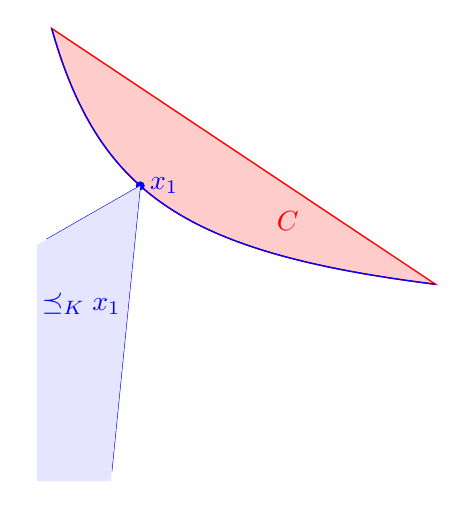
\begin{tikzpicture}
  \begin{axis}[
    ticks=none,
    y=3cm,            % y unit vector
    x=1.5cm,
    % hide y axis,        % hide the y axis
    axis lines = none,
    x label style={at={(axis description cs:0.5,0.1)},anchor=north},
    y label style={at={(axis description cs:0.25,0.5)},anchor=south},
    clip=false
    ]

    \addplot[fill=red!20, draw=red, line width = 0.5pt, domain=-0.75:2.5, samples=200]{1/(x+1.5)-1/1.5}--cycle;

    \addplot[draw=blue, line width = 0.5pt, domain=-0.75:2.5, samples=200]{1/(x+1.5)-1/1.5};

    \node [circle, draw=blue, fill=blue, inner sep=1pt] (x1) at (axis cs:0,0) {};
    \node [right, blue] at (x1) {$x_1$};

    \node at (axis cs:-3.5/4,-1/4) (b) {};
    \node at (axis cs:-1/4,-5/4) (c) {};

    \draw[blue] (axis cs:0,0)--(b);
    \draw[blue] (axis cs:0,0)--(c);

    \fill [blue!10] (axis cs:0,0) -- (b.center) -- (axis cs:-3.5/4,-5/4)  -- (c.center) -- cycle;

    \node [blue] at (axis cs:-0.5,-0.5) {$\preceq_K x_1$};
    \node [red] at (axis cs:1.25,-.15) {$C$};

  \end{axis}
\end{tikzpicture}

\end{document}

%%% Local Variables:
%%% mode: latex
%%% TeX-master: t
%%% End:
